
%% notes on k-means
%%

\minitoc

In this lecture we will take a detour and introduce the \href{https://en.wikipedia.org/wiki/K-means_clustering}{k-means algorithm} for clustering data. For more details on clustering algorithms and the Loyd's k-means algorithm in particular see Chapter 4 of ``Introduction to Applied Linear Algebra: Vectors, Matrices, and Least Squares'' \cite{boyd2018introduction} [ available to download  \href{http://vmls-book.stanford.edu/vmls.pdf}{here}]. In the class you will first implement this with a serial C code, then add threaded parallelism with OpenMP, and finally convert it to work with the Message Passing Interface for distributed computing. This will enable you to perform clustering on progressively larger and larger problems as you switch from computing on your laptop with serial C, to computing on a workstation with OpenMP on multiple CPU cores, to computing on a cluster with MPI running between multiple compute nodes.

\section{Voronoi diagrams}

{\bf Note}: you do not need to explicitly find the Voronoi diagram in your \texttt{kmeans} code. This section is provided as motivational background on how the k-means algorithm works.

Before we dive into the k-means algorithm we introduce the \href{https://en.wikipedia.org/wiki/Voronoi_diagram}{Voronoi diagram} which is named after Georgy Voronoi who formulated them for arbitrary dimensional spaces. For more on the history see    \href{https://en.wikipedia.org/wiki/Voronoi_diagram}{Voronoi diagram wiki page}. 

{\bf Definition}: Given a set of points in d-dimensional space, a Voronoi diagram consists of a set of polytopes (we will call these cells from now on) that partition the domain such that each cell encloses just one of the points. Furthermore, the cells have the property that any point on the border of one or more cells is equidistant from the points contained within those cells.

{\bf Implementations}: MATLAB has a built in \texttt{voronoi} function that build a Voronoi diagram and plots it. There is also a collection of implementations of the Voronoi in different programming languages at \href{https://rosettacode.org/wiki/Voronoi_diagram}{rosettacode.org}.


\begin{figure}[htbp!]
    \centering
    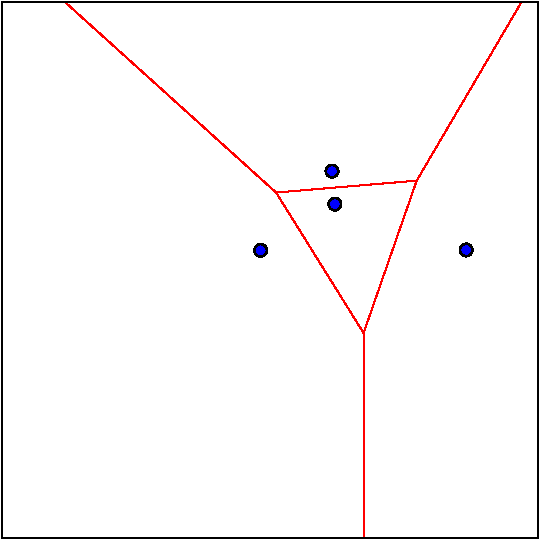
\includegraphics[width=0.22\textwidth]{figures/kmeans/voronoiRand4-crop.pdf}
    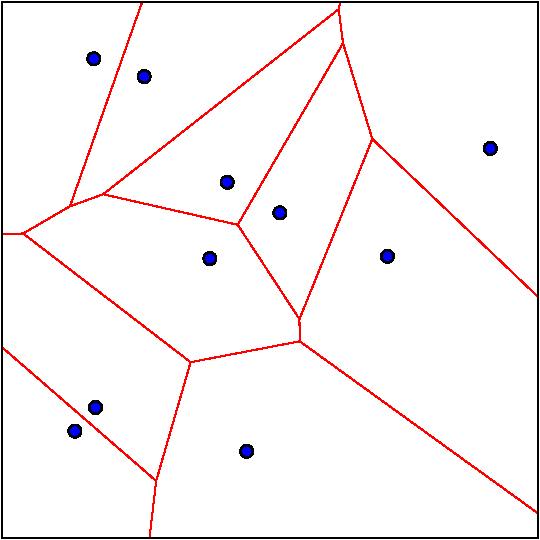
\includegraphics[width=0.22\textwidth]{figures/kmeans/voronoiRand10-crop.pdf}
    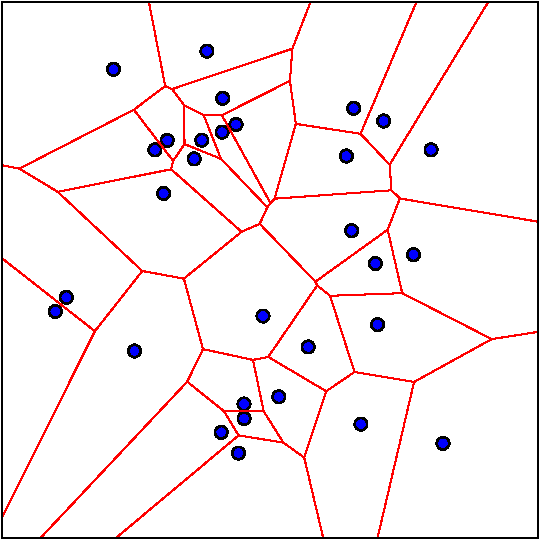
\includegraphics[width=0.22\textwidth]{figures/kmeans/voronoiRand30-crop.pdf}
    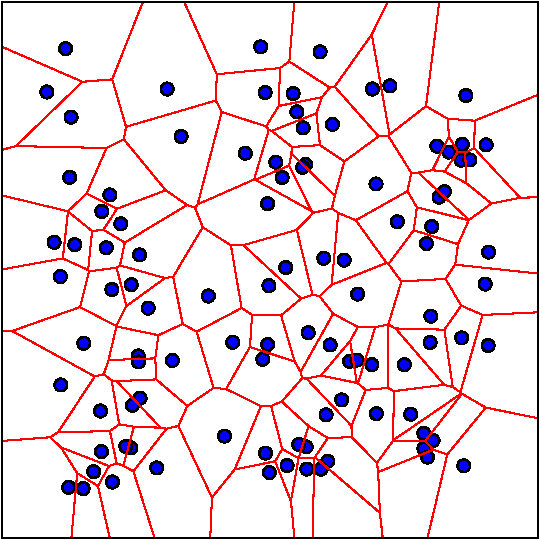
\includegraphics[width=0.22\textwidth]{figures/kmeans/voronoiRand100-crop.pdf}
    \caption{Voronoi diagrams for point sets with $N=4,10,30,$ and $100$ randomly chosen points. The red lines for the body of the Voronoi cells. The blue circles are the randomly chosen data points. }
    \label{voronoiExamples.fig}
\end{figure}

{\bf Examples}: In Figure \ref{voronoiExamples.fig} we show Voronoi diagrams for four randomly chosen sets of $N=4,10,30,$ and $100$ data points . It should be apparent that the Voronoi diagrams satisfy the following properties

\begin{enumerate}
\item Each Voronoi cell has linear sides.
\item Each Voronoi cell contains one and only data point. 
\item Each Voronoi cell is convex.
\item Any point chosen inside a cell is closer to the blue data point contained inside the cell than any other data point outside the cell.
\end{enumerate}

We will use Voronoi diagrams in the follow sections as an implicit way to partition a domain as part of Lloyd's algorithm for the k-means clustering problem. In the ideal case data points that cluster nearby will reside within one cell of a Voronoi diagram. For instance, imagine the case where the random data points in Figure \ref{voronoiExamples.fig} actually represent centers of regions where there are tightly clusters groups of data, then indeed the Voronoi diagram does a reasonable job of partitioning the data geometrically since all the points in the vicinity of the blue dots will be closer to each other than to the data in the other cells.


\section{Cluster notation}

We will need some notation to set the stage for geometric clustering of data points. First let's assume we have $N$ data points and that data point with index $i$ has coordinates $(x_i,y_i)$. Our goal is to assign an integer label $c_i$ to data point $i$ for $i=0,\ldots,N-1$. This will assert an affinity between the data point and cluster group. All data points associated with the same cluster will have the same label, i.e. if $c_1 = c_{10}$ then data points 1 and 10 will be considered to be in the same group. Moreover the integer values of $c_i$ must be in the range $[0,K)$\footnote{Note the use of the brackets on the interval $[0,K)$. The round bracket excludes $K$ and the square bracket  includes $0$.}

We will need to be able to compute the centroid of data points in each cluster. To do this we can compute moments of the data relative to the cluster groups as follows. 

The zero moment, sometimes known as the cardinality of the groups is computable for cluster $k$ with the following formula cluster defined by
\[
C_k := \sum_{i=0}^{i=N-1} \delta_{k,c_i},
\]
which you will recognize after a moment's reflection as the number of data points assigned to cluster with label $k$ (since the quantity in the summation is one if the point is in cluster $k$ or zero otherwise). Here $\delta_{a,b}$ denotes the Kronecker delta given by
\[
\delta_{a,b} = \left\{ \begin{array}{l} 1\;\mbox{if}\;a=b, \\
0\;\mbox{otherwise}.
\end{array}\right.
\]
The first moment, sometimes known as the centroid of  cluster $k$ is computed by
\begin{eqnarray}
\hat{x}_k & := & \frac{1}{C_k} \sum_{i=0}^{i=N-1} x_i\delta_{c_i,k},\\ \hat{y}_k & := & \frac{1}{C_k} \sum_{i=0}^{i=N-1} y_i\delta_{c_i,k},
\end{eqnarray}
and you can think of this as the geometric center of the data points that have label $k$.

The k-means clustering problems seeks to group data points into $K$ clusters. That means we must choose an integer numerical labelling of the nodes (i.e. choose $c_i\in 0, \ldots, K-1$ for $i \in 0, \ldots, N-1$) that minimizes the total sum of squares of the the distances between the data points and the centroids of their assigned cluster given by this formula
\[
d:=\sum_{i=0}^{i=N-1} \left( (x_i - \hat{x}_{c_i})^2 + (y_i - \hat{y}_{c_i})^2 \right)
\]
In words: we want to assign the data points to cluster in a way that collectively minimizes the variance of the data points from their assigned cluster centroids. 

In general this is a so-called NP hard problem. This means to guarantee we have actually found a globally optimal clustering is as computationally expensive as the hardest problem in the equivalence class of NP hard problems and it is  likely that computational cost of exhaustively solving this optimization problem increases faster than any polynomial in $N$ (unless \href{https://en.wikipedia.org/wiki/NP-hardness}{P=NP}).

Since this is a computationally hard problem we will resort to a \href{https://en.wikipedia.org/wiki/Heuristic}{heuristic method}. In this context ``heuristic'' means that the method is found to work well in practice but is not guaranteed to always produce nearly optimal clusters and/or may sometimes take a very long time to finish.

\newpage
\section{Lloyd's clustering algorithm}

We will focus on the relatively simple heuristic clustering algorithm due to Lloyd \cite{lloyd1982least}. It was first described in a technical report in 1957 but not published since the computations were not complete until 1982. The idea is simple but also really clever and I will describe it in two parts in pseudo-code. 

\subsection{Assign data points to cluster by proximity to their centroids}
In the first stage of Lloyd's algorithm we assume that initial cluster labels and corresponding centroids are provided. Then for each node we find the closest centroid to $(x_i,y_i)$ and the index of the closest centroid is the new cluster label $c_i$. 

\begin{algorithm}[htbp!]
\caption{Lloyd's clustering algorithm: assignment to cluster}\label{lloydAssignment.alg}
\vspace{4pt}
\KwInput{$N,K\in\mathbb{N}$}
\KwInput{$x,y\in \mathbb{R}^N$}
\KwInput{$\hat{x},\hat{y}\in \mathbb{R}^K$}
\KwOutput{$c\in \mathbb{N}^N$}
\KwRequire{$0\leq c_i < K$}
\algrule
\For{$i\in [0,N)$}{
  $c_i =\argmin\limits_{k\in 0,\ldots,K-1}\left( (x_i - \hat{x}_k)^2+ (y_i - \hat{y}_k)^2 \right)$
  }
\end{algorithm}

\newpage
\subsection{Compute cluster centroids}

In the second part of Lloyd's algorithm we compute the centroids for the newly reassigned clusters from the first algorithm. This algorithm will compute centroids for each label in $[0,K)$. If there is an empty cluster it will assign random coordinates to the centroid of the empty cluster.

\begin{algorithm}[htbp!]
\caption{Lloyd's clustering algorithm: recompute centroids}\label{lloydCentroid.alg}
\vspace{4pt}
\KwInput{$N,K\in\mathbb{N}$}
\KwInput{$x,y\in \mathbb{R}^N$}
\KwInput{$c\in \mathbb{N}^N$}
\KwOutput{$\hat{x},\hat{y}\in \mathbb{R}^K$}
\KwRequire{$0\leq c_i < K$}
\algrule
 \For{$k\in [0,K)$}{
   $\hat{x}_k = 0$\; $\hat{y}_k = 0$\; $C_k = 0$\;
 }
 \For{$i\in [0,N)$}{
    $j:=c_i$\;
    $\hat{x}_j = \hat{x}_j + x_i$\;
    $\hat{y}_j = \hat{y}_j + y_i$\;
    $C_j = C_j + 1$\;
  }
  \For{$k\in [0, K)$}{
    \If{$C_k = 0$}{
      $\hat{x}_k = \hat{x}_k/C_k$\; $\hat{y}_k = \hat{y}_k/C_k$\;
    }
    \Else{
      $\hat{x}_k = \mbox{drand}()$\; $\hat{y}_k = \mbox{drand}()$\;
    }
}
\end{algorithm}

\newpage
\subsection{Lloyd's clustering algorithm}
We put the two Algorithms together and repeat  in the following pseudo-code for the overall Lloyd's algorithm

\begin{algorithm}[htbp!]
\caption{Lloyd's clustering algorithm}
\label{lloyd.alg}
\vspace{4pt}
\KwInput{$N,K\in\mathbb{N}$}
\KwInput{$x,y\in \mathbb{R}^N$}
\KwInput{$\mbox{tol}\in \mathbb{R}$}
\KwInputOutput{$c\in \mathbb{N}^N$}
\KwRequire{$0\leq c_i < K$}
\algrule
 \While{centroid change exceeds tol}{
   Algorithm 1: assign each datapoint to cluster with nearest centroid \;
   Algorithm 2: recompute centroids of clusters \;
   Compute maximum change of centroids \;
 }
\end{algorithm}

For the rest of the semester you will revisit this algorithm multiple times. Initially you will implement this in C as part of Assignment 07.

\printbibliography[heading=subbibliography]